% last updated in April 2002 by Antje Endemann
% Based on CVPR 07 and LNCS, with modifications by DAF, AZ and elle, 2008 and AA, 2010, and CC, 2011; TT, 2014

\documentclass[runningheads]{llncs}
\usepackage{graphicx}
\usepackage{amsmath,amssymb} % define this before the line numbering.
\usepackage{ruler}
\usepackage{color}
\usepackage[width=122mm,left=12mm,paperwidth=146mm,height=193mm,top=12mm,paperheight=217mm]{geometry}


\usepackage{times}
\usepackage{epsfig}
\usepackage{graphicx}
\usepackage{amsmath}
\usepackage{amssymb}
\usepackage{url}
\usepackage{bm}


\begin{document}

%\psdraft



% \renewcommand\thelinenumber{\color[rgb]{0.2,0.5,0.8}\normalfont\sffamily\scriptsize\arabic{linenumber}\color[rgb]{0,0,0}}
% \renewcommand\makeLineNumber {\hss\thelinenumber\ \hspace{6mm} \rlap{\hskip\textwidth\ \hspace{6.5mm}\thelinenumber}}
% \linenumbers
\pagestyle{headings}
\mainmatter
\def\ECCV14SubNumber{321}  % Insert your submission number here

\title{Clouds in The Cloud} % Replace with your title

\titlerunning{ECCV-14 submission ID \ECCV14SubNumber}

\authorrunning{ECCV-14 submission ID \ECCV14SubNumber}

\author{Anonymous ECCV submission}
\institute{Paper ID \ECCV14SubNumber}


\maketitle

\begin{abstract}
abstract
\end{abstract}

%%%%%%%%%%%%%%%%%%%%%%%%%%%%%%%%%%%%%%%%%%%%%%%%%%%%%%%%%%%%%%
\section{Introduction}
\label{sec:intro}

Following the introduction of plenotic imaging to computer vision, light-field imaging~\cite{bishop,horstmeyer,levoy,kim} has had a significant impact on sensing. This modality samples the radiance distribution in location and direction. It has so far been used mainly in small-scale setups. However, it can be scaled up to continental size, to map the Earth's atmosphere in 3D. Sampling the atmospheric radiance in spatio-angularly is achieved by a few spaceborne and airborne instruments, including the Multiangle Imaging SpectroRadiometer (MISR)~\cite{diner,matronchik}, the Airborne Multiangle SpectroPolarimetric Imager (AirMSPI)~\cite{dinerDavis07,dinerDavis10} and POLDER~\cite{baxter,breon,vanMol}.
However, these imaging architectures suffer several drawbacks. They have crude resolution spatially (effectively several kilometers per pixel), angularly  ($\approx 7$ angles per view), and temporally (orbit takes several days to return to the same terrestrial spot). Furthermore, spaceborne instruments are extremely expensive and unscalable. Hence, in this work we develop a counter approach: the atmospheric lightfield is captured {\em from below}, by wide-angle cameras {\em looking upwards}. Moreover, instead of expensive one-off instruments, our approach is a {\em scalable sensor network} that captures images simultaneously over an a very large area, densely.

Creating and exploiting such a light-field imaging-network poses several requirements: low-cost units,
communications, and {\em tailored computational photography algorithms}. The first two requirements are met  thanks to cellular-network infrastructure, cellular-based low-cost cameras and {\em cloud computer} servers. Hence, we can deploy solar-powered cameras at will, nearly anywhere, and they upload their sky-images to the cloud, from which the light-field data are analyzed. However, this new type of imaging-system gives rise to new problems and algorithms, part of which we deal with in this paper. In a sense, the network {\em generalizes compute vision problems} that had been posed for single-camera, a decade ago. On the other hand, network redundancy offers {\em solutions} to these problems.

The computational photography problems include radiometric self-calibration across a network of low-cost cameras, geometric calibration in the field, and overcoming flare by a network. Consequently, the light-field network enables unprecedented 3D imaging of clouds, in high spatio-temporal resolution. This is achieved by expanding {\em space carving} to {\em volumetric distribution} of semi-transparent clouds. We demonstrate the approach using real field experiments, based on a network of five cameras. As a result, we believe this approach can complement multi-angular satellite cloud imagery, and perhaps make aerosol tomography~\cite{aides} realizable.



%%%%%%%%%%%%%%%%%%%%%%%%%%%%%%%%%%%%%%%%%%%%%%%%%%%%%%%%%%%%%%
\section{Background}
\label{sec:theory}

%%%%%%%%%%%%%%%%%%%%%%%%%%%%%%%%%%%%%%%%%%%%%%%%%%%%%%%%%%%%%%
\subsection{Single-camera radiometric self-calibration}
\label{sec:Signelradio}

To create a large network of cameras, each camera unit should have low cost. Such digital cameras often have inconsistent radiometric problems of gain, white balance etc. For a single camera, consistent readouts can be obtained by self-calibration. The strongest methods rely on redundant images, taken at different settings. In particular, images taken at different exposure times calibrate the radiometric response, up to a global scale factor. Similarly, images taken by slowly panning the camera yields spatial non-uniformity correction (NUC). In particular, nonuniformity (e.g., by vignetting~\cite{kang}) is often modeled by a function $M({\bf x})$, where \mbox{${\bf x}=(x,y)$} is a camera pixel. Thus the image pixel irradiance at time $t$ is
\begin{equation}
 \tilde{I}_t({\bf x}) = M({\bf x})I_t(O) \;,
 \label{eq:tilde_I}
\end{equation}
where $I(O)$ is the pixel irradiance when $M=1$, for observed object $O$. Let the camera be panned, so that the object $O$ projects to pixel ${\bf x}'$ in time $t'$.
{\em Correspondence} is established between the two pixels, by image alignment. This yields a redundant measurement $\tilde{I}_t'({\bf x}') = M({\bf x}')I_t'(O)$. Assuming brightness constancy, $I_t(O)=I_t'(O)$, the two measurements yields a linear constraint
\begin{equation}
 \log M({\bf x})- \log M({\bf x}')=\log \tilde{I}_t({\bf x})-\log \tilde{I}_t'({\bf x}').
 \label{eq:logM}
\end{equation}
Aggregating many such constraints over different pixels and frames recovers $M({\bf x})$, up to a global exponential ambiguity. This recovery makes pixel readout spatially consistent. Similar formulations exist for additive spatial nonuniformity, or for camera gain (yielding temporal consistency).
In Sec.~\ref{sec:mutiradio} we expand this principle to a camera-array.


%%%%%%%%%%%%%%%%%%%%%%%%%%%%%%%%%%%%%%%%%%%%%%%%%%%%%%%%%%%%%%
\subsection{Avoiding Blooming, Lens-Flare in a Single Camera}
\label{sec:Signelflare}

A wide-angle camera observing the sky is liable to frequently have sun-rays shine directly into the lens system. This creates problems. First, saturation in pixels to which the sun project creates blooming. Blooming by direct sunlight challenges the sensor even in high-dynamic range setups. Second, the sun-rays creates lens-flare, which is an additive spatially varying image component. Computational photography methods suggested were suggested to reduce lens flare: images can be taken by a specialized detector array. Alternatively, sharp flare features (but not global bias) can be eliminated by rotating the camera and taking consecutive frames, but the scene might change by then. Both approaches hinder the need for simple, low-cost solution and operation.
%Third, direct sunlight repeatedly entering the camera chamber and hitting pixels may damage the camera after a while.

Consequently, for sky-observing wide-field cameras, the most common solution to all these problems is a {\em dynamic sun blocker}. It is a essentially an opaque piece raised above the camera optics, in the direction of the Sun, blocking the Sun and the sky around. There are various configurations, but all of them need to {\em move}, as the Sun direction changes during the day and across the year. Motorized solutions that need to work year-around significantly complicate such camera units, making them very expensive. In Sec.~\ref{sec:mutiSun} we show that a large camera network inherently bypasses the problem, without a need to constantly move a Sun blocker.





%%%%%%%%%%%%%%%%%%%%%%%%%%%%%%%%%%%%%%%%%%%%%%%%%%%%%%%%%%%%%%
\subsection{Current 3D Cloud Mapping}
\label{sec:current3D}


Existing scientific\footnote{There are also ground viewing webcams that happen to see sky parts~\cite{bradley} and weather cameras
that are too sparse to be integrated for recovery.} sky-imaging systems use a handful of high quality cameras~\cite{allmen,baumgarten,cazorla,long,Seiz,kassianov}. Due to their complexity and costs, they were only operated to estimate {\em cloud-base} over narrow regions right above a narrow-baseline camera pair. Satellite-based estimation of 3D {\em cloud-tops} has been proposed by MISR. To measure clouds above a specific region, it takes several minutes for MISR to reach each of the seven viewpoints on the orbit track, during which the clouds generally move.


%%%%%%%%%%%%%%%%%%%%%%%%%%%%%%%%%%%%%%%%%%%%%%%%%%%%%%%%%%%%%%
\subsection{Space Carving}
\label{sec:photohull}

Space carving is a method to constrain a hull of a 3D opaque object. Iterating from an initial hull shape estimation, its different voxels are projected to cameras at several viewpoints. If projections of a voxel are photometrically inconsistent in the different cameras, then this voxel is carved-out from the estimated object.



%%%%%%%%%%%%%%%%%%%%%%%%%%%%%%%%%%%%%%%%%%%%%%%%%%%%%%%%%%%%%%
\section{Self-Calibration in a Camera Network}
\label{sec:muticalib}

Consider a network of cameras units, each of which has somewhat loose quality control, for lower cost-per-unit. Then, there might be radiometric inconsistencies between cameras, i.e., the same distant object has different intensity readouts for different cameras. Estimating and then compensating for inter-camera differences is helpful for subsequent computer vision algorithms. It is clear that radiometric consistency is necessary for radiometric-based tasks, such as aerosol tomography. However, it also assists non-radiometric, higher level tasks. For example, suppose we seek to segment clouds over the sky background. Segmentation has to be as consistent as possible across the different viewpoints, lest voxel association to clouds have contradictions between camera subsets. To achieve this, image-value thresholds that might be used for segmentation need to be mutually consistent.

Similarly to Sec.~\ref{sec:Signelradio}, the solution relies on redundant measurement at {\em corresponding} points.   For correspondence, geometric calibration is a first necessity. Thus, we first this step, which relies on ideas from Refs.~\cite{gemetricsky}.

%%%%%%%%%%%%%%%%%%%%%%%%%%%%%%%%%%%%%%%%%%%%%%%%%%%%%%%%%%%%%%
\subsection{Geometric calibration}
\label{sec:geometry}

The cameras are independently deployed in the field. For each camera $c$, its location vector ${\bf l}_c$ is known by GPS, and the internal parameters $\Psi_c$ are pre-calibrated in the lab. However, the orientation (yaw, pitch and roll angle vector ${\bf \Theta}_c$) is loosely set, as the camera is placed in the field. We calibrate the orientation by detecting and tracking extra-terrestrial (XT) objects (Sun and/or Moon), across day or night in the hemispherical field of view. Using astronomical charts per time $t$ and ${\bf l}_c$, an XT object is known to be at angle vector (zenith, azimuth) ${\bm \theta}^{\rm XT}(t)$ relative to a global coordinate system. Given camera orientation ${\bf \Theta}_c$, a ray from
${\bf \Theta}^{\rm XT}(t)$ should project to pixel
\begin{equation}
{\bf x}^{\rm XT}_{\rm model}(t) = {\cal P}({\bm \theta}^{\rm XT}(t)|{\bf \Theta}_c,\Psi_c)
\;,
 \label{eq:xt}
\end{equation}
where ${\cal P}$ is a projector operation (converting ray angles to image pixels).
The actual measured pixel ${\bf x}^{\rm XT}_{\rm measured}(t)$ has uncertainty to the finite angular size of the XT object and blooming. However, during the course of a day or night, the number of frames
  $N^{\rm frames}$ is in the hundreds, leading to a simple optimization formulation.
\begin{equation}
 \hat{\bf \Theta}_c=\arg\min_{{\bf \Theta}_c}
 \sum_{t=1}^{N^{\rm frames}}
 \|{\cal P}({\bm \theta}^{\rm XT}(t)|{\bf \Theta}_c,\Psi_c) - {\bf x}^{\rm XT}_{\rm measured}(t)\|^2
\;,
 \label{eq:hatThetac}
\end{equation}

To test the hypotheses of this paper, we built a small experimental network. To show that it can work with very low-cost  camera nodes (units), each of the 5 units was built from basic components, and coarse alignment tolerances. Its core is a Raspberry-Pi computer used in DIY electronics, and a 5MP Raspberry-Pi camera. We cut-off its OEM lens, and manually attached a small fisheye lens to it. Due to this coarse lens-to-chip
alignment {\bf each camera has a different peripheral dead-region}, creating a missing part in the hemispheric view-field and vignetting distinct to each camera. As derived below, a {\em {\bf network} as-a-whole can {\bf inherently overcome}} these issues. Every 30 seconds, in synchrony, all units automatically transmitted their data using the cellular network to a {\em cloud-computer server}. Each unit was solar powered (Fig.~\ref{fig:system}).
\begin{figure}[t!]
\begin{center}
   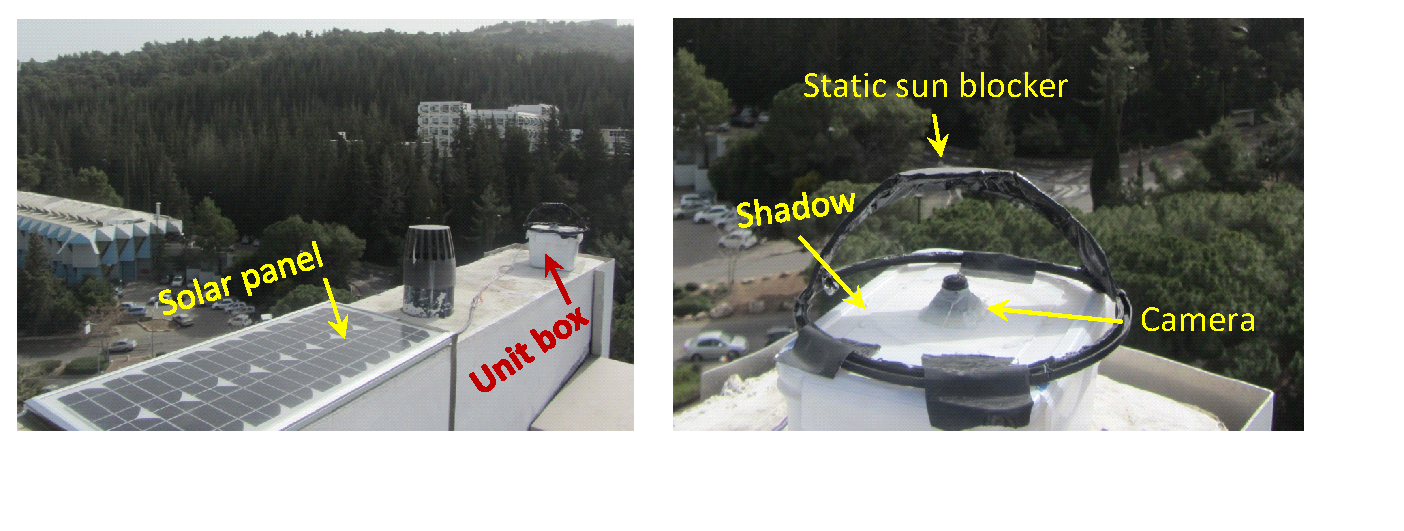
\includegraphics[width=1\linewidth]{figures/system.eps}
\end{center}
   \vspace{-0.6cm}
   \caption{(A unit (network-node) on a rooftop in a hilly area. It is solar powered. 
   It encapsulates a Raspberry-Pi camera. Its fisheye lens is shadowed here by a mounted  static Sun-blocker.
   }
\label{fig:system}
\end{figure}
The orientation calibration is illustrated in Fig.~\ref{fig:sunmotion}.
\begin{figure}[t!]
\begin{center}
   \includegraphics[width=1\linewidth]{figures/sun_moon.eps}
\end{center}
   \vspace{-0.6cm}
   \caption{(a) To estimate the yaw-pitch-roll angle vector ${\bf \Theta}$ of camera $c$), we rely on
   image locations of extra-terrestrial objects, whose direction vector ${\bm \theta}^{\rm XT}(t)$
   in known for all time $t$. (b) Photo-montage of the daylight sky. It shows the Sun at different hours, the expected trajectory based on the estimated ${\bf \Theta}$, and lens-flares. (c)
   Photo-montage of night sky images. It shows the moon at different times, the expected trajectory based on the estimated ${\bf \Theta}$, and a close-up on the corresponding sampled images of Jupiter.}
\label{fig:sunmotion}
\end{figure}


Based on $\hat{\bf \Theta}_c$, all captured images $\tilde I_{c,t}(\bf x)$ taken by camera $c$ are aligned to the global coordinate system. Any image pixel ${\bf x}$ of camera $c$ is backprojected to a ray at angle and direction vector ${\bm \theta}(c)$ in the global system, given by
\begin{equation}
 {\bm \theta}_c(\bf x)={\cal P}^{-1}({\bf x}|\hat{\bf \Theta}_c,\Psi_c)
  \;.
 \label{eq:thetac}
\end{equation}
The sampled light-field is the radiance measured per location, direction and time, thus given by
$\tilde I_t[{\bf l}_c,{\bm \theta}_c(\bf x)]$.
\begin{figure}[t!]
\begin{center}
   \includegraphics[width=1\linewidth]{figures/scence_c.eps}
\end{center}
   \vspace{-0.6cm}
   \caption{Images taken simultaneously by a 5-node network. They are geometrically aligned to the zenith and north, and resampled to {\em polar azimuthal equidistant} projection in this global system. Equidistant zenith angle circles are overlayed on $\tilde I_t[{\bf l}_e,{\bm \theta}]$ (camera $e$). Each camera has dead-regions, since the lens-axis had only roughly been centered on the board of our tiny DIY units.
   Corresponding to the frame in camera $e$, a {\em cloud score} map (Eq.~\ref{eq:sr}) has high values in cloud-pixels, diminishing outside them. [Bottom-right] The 3D setup of the experimental network. It is laterally spread over several hundreds of meters, on rooftops at somewhat different heights.}
\label{fig:photomotion}
\end{figure}


%%%%%%%%%%%%%%%%%%%%%%%%%%%%%%%%%%%%%%%%%%%%%%%%%%%%%%%%%%%%%%
\subsection{Radiometric Self-Calibration in a Camera Network}
\label{sec:mutiradio}

%
%%%%%%%%%%%%%%%%%%%%%%%%%%%%%%%%%%%%%%%%%%%%%%%%%%%%%%%%%%%%%%%
%\subsection*{The Experimental Setup}
%\label{sec:system}
%

Consider a {\em fixed} view direction ${\bm \theta}$ observed in several cameras.
%, e.g., $c$ and $c'$.
The values $\{\tilde I_t[{\bf l}_c,{\bm \theta}]\}_c$ correspond to readouts of parallel rays back projected from all cameras in the network. The values in this set generally different from each other, e.g.,
 $\tilde I_t[{\bf l}_c,{\bm \theta}]\neq \tilde I_t[{\bf l}_{c'},{\bm \theta}]$. There are two causes for this difference:\\
 {\tt 1}.~ Different camera locations mean different observed objects. Momentarily, camera $c$ may observe a cloud while $c'$ observes a clear sky, or vice versa. Camera $c'$ may momentarily observe a somewhat denser haze volume than $c$, or vice versa. \\
 {\tt 2}.~ Slight inter-camera radiometric inconsistencies, which we need to estimate.\\
 Cause {\tt 1} is usually dominant. We need to overcome it, in order to get analyze cause {\tt 2}.

The assumption we make is of {\em regional stationarity}. In a region containing the cameras, the chance of a cloud, clear sky, or haziness affecting $\tilde I_t[{\bf l}_c,{\bm \theta}]$ is {\em independent} of $c$.
Thus, inter-camera image variations due to atmospheric conditions are {\em random and unbiased}. Per camera $c$ and view angle ${\bm \theta}$, bias is due to cause {\tt 2}. We easily detect and characterize the bias by capturing {\em statistics over time}.

Consider, for example, Fig.~\ref{fig:calibration}. It shows [Top-Left] radiometric inconsistency between cameras $a$ and $b$. The figure then shown a scatter-plot of
$\tilde I_t[{\bf l}_a,{\bm \theta}]$ vs.~$\tilde I_t[{\bf l}_{b},{\bm \theta}]$, $\forall t,{\bm \theta}$, for the red-channel.
\begin{figure}[t!]
\begin{center}
   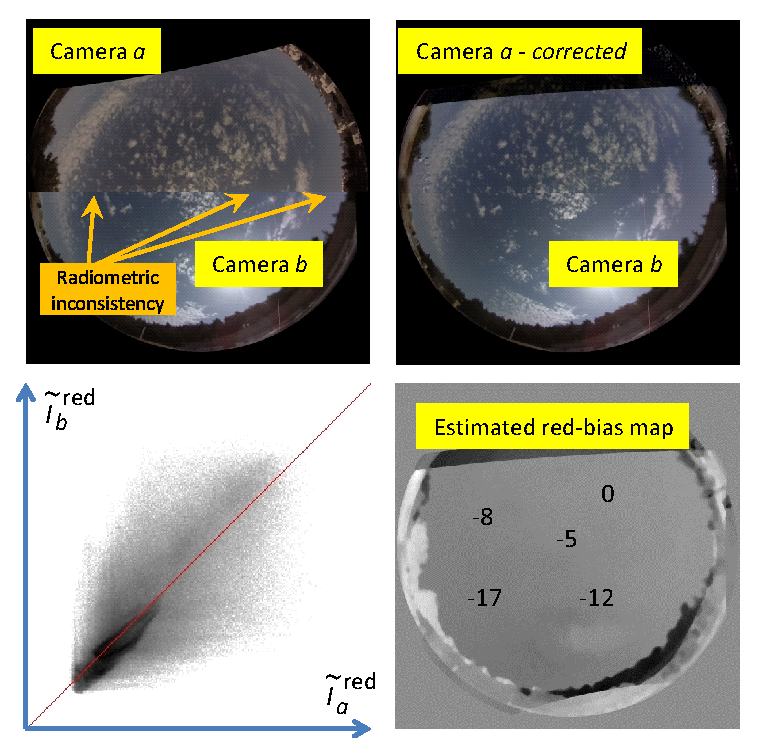
\includegraphics[width=0.6\linewidth]{figures/bias1a.eps}
\end{center}
   \vspace{-0.6cm}
   \caption{[Top-Left] Splitting the field of view in half, to pixels from either
   $\tilde I_t[{\bf l}_a,{\bm \theta}]$  or $\tilde I_t[{\bf l}_{b},{\bm \theta}]$. Radiometric inconsistency
   shows-up as a seam-line across which colors slightly change. [Bottom-Left] Scatter-plot of
   $\tilde I_t[{\bf l}_a,{\bm \theta}]$ vs.~$\tilde I_t[{\bf l}_{b},{\bm \theta}]$, $~\forall t,{\bm \theta}$, red-channel. [Bottom-right] The estimated offset map ${\hat o}_{b-a}({\bm \theta})$, red channel. It is derived based on a set of images taken during several hours.
   [Top-right] Splitting the field of view in half, to {\em corrected} pixels from either
   $\hat I_t[{\bf l}_a,{\bm \theta}]$  or $\hat I_t[{\bf l}_{b},{\bm \theta}]$: inconsistencies are greatly
   diminished.
   }
\label{fig:calibration}
\end{figure}
From this scatter plot and those of the other color channels, we hypothesized that camera $a$ has a slight offset, particularly in the red channel, relative to camera $b$. We thus estimated, per color channel, the
map of radiometric offset (across pixels, ray directions).
To handle outliers, a temporal median was used
\begin{equation}
 {\hat o}_{b-a}({\bm \theta})=
  {\rm median}_{t} \{\tilde I_t[{\bf l}_b,{\bm \theta}]-I_t[{\bf l}_a,{\bm \theta}]\}
 \label{eq:hato}
\end{equation}
The map ${\hat o}_{b-a}({\bm \theta})$ was then spatially smoothed and used to correct $\tilde I_t[{\bf l}_a,{\bm \theta}]$. As shown in Fig.~\ref{fig:calibration}, the results have much better inter-camera consistency, and this this was apparent in images taken throughout that day. A similar process was applied to other cameras, but they had negligible radiometric inconsistencies with respect to camera $b$. After radiometric corrections, the light-field samples are denoted tilde $\hat I_t[{\bf l}_b,{\bm \theta}]$.





%%%%%%%%%%%%%%%%%%%%%%%%%%%%%%%%%%%%%%%%%%%%%%%%%%%%%%%%%%%%%%
\section{Network-assisted Background Estimation}
\label{sec:background}

To detect clouds, it is often helpful to characterize the background, as is typical in change-detection computer vision algorithms. In monocular settings, such algorithms use temporal filtering to characterize the background: foreground dynamic objects are at {\em different locations at different times} and are thus pruned. In our case this translates to stating that a cloud in
$\tilde I_t[{\bf l}_c,{\bm \theta}]$ is often not in
$\tilde I_{t'}[{\bf l}_c,{\bm \theta}]$, when $t'\neq t$. However, if clouds move slowly, while illumination gradually changes, temporal filtering may be insufficient. This is illustrated in Fif

A light-field network enhances this principle, with more effective pruning-per-time. After calibration, {\em simultaneous} images captured by {\em different camera nodes} are different from each other. Thus, change of viewpoint has an effect similar to change in time: a cloud in
$\tilde I_t[{\bf l}_c,{\bm \theta}]$ is often not in $\tilde I_t[{\bf l}_{c'},{\bm \theta}]$. This principle relies on the {\em regional stationarity} mentioned above. Consequently, background sky values are obtained by data filtering over both time and viewpoint.

In broad daylight, clouds are brighter than the blue sky. Hence, an estimator for the sky background is
\begin{equation}
 {\rm SKY}({\bm \theta})= \arg\min_{t,c} \tilde I_t[{\bf l}_c,{\bm \theta}]
 \label{eq:SKY}
\end{equation}
where $t\in[1\ldots N^{\rm frames}]$ and $c\in[1\ldots N^{\rm views}]$.
This is illustrated in Fig.~\ref{fig:sky}.
\begin{figure}[t!]
\begin{center}
   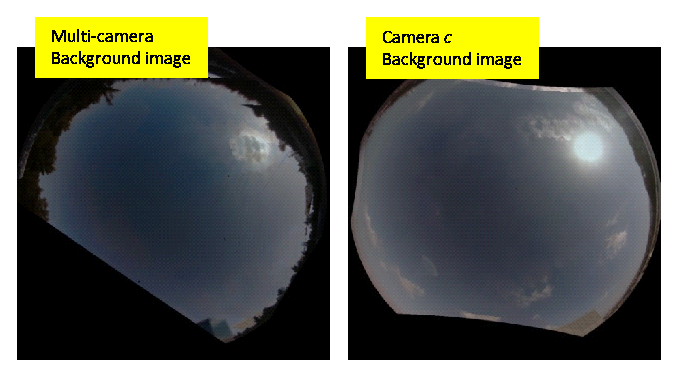
\includegraphics[width=0.6\linewidth]{figures/Background.eps}
\end{center}
   \vspace{-0.6cm}
   \caption{[Left] Estimation of the sky background, using Eq.~(\ref{eq:SKY}) based on 5 temporal
   instances and 5 viewpoints. [Right] Estimation of the sky background, using 5 temporal
   instances, but just a single viewpoint, resulting in more residual clouds.}
\label{fig:sky}
\end{figure}


%%%%%%%%%%%%%%%%%%%%%%%%%%%%%%%%%%%%%%%%%%%%%%%%%%%%%%%%%%%%%%
\section{Bypassing the Sun through a Camera Network}
\label{sec:mutiSun}

As Sec.~\ref{sec:Signelflare} explains, in existing full sky-imagers, effects of direct sunlight are mitigated by a small dynamic sun-blocker, which complicates the system and its cost, while having a blind-region. The network offers a different solution, which can be radical, yet simple. On each camera, the sun-blocker is {\em static}, and has no moving part. The blocker can be large, covering the entire range of directions the Sun may occupy during the year. In this configuration, each camera unit has a large blind area (See Fig.~\ref{fig:blindspot}). Nevertheless, the entire {\em network has no blind spot}, when viewing the atmosphere. This remarkable property is a result of network-redundancy, as we explain.
\begin{figure}[t!]
\begin{center}
   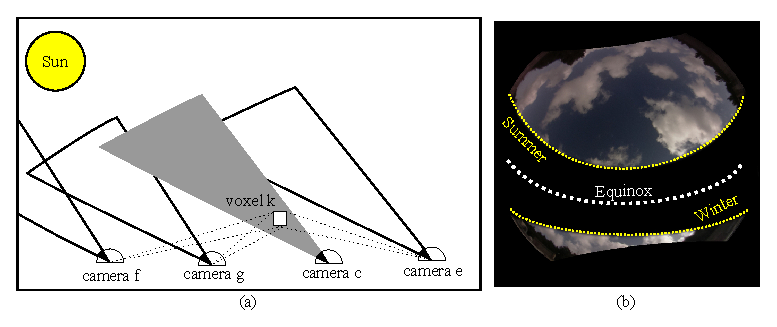
\includegraphics[width=1\linewidth]{figures/sun_blocks.eps}
\end{center}
   \vspace{-0.6cm}
   \caption{Camera $c$ has a blind-region, covering Sun directions at ${\bf l}_c$. The blind region corresponds to set $\Gamma_c$ of atmospheric voxels not sensed by by camera $c$. The network as a whole still has coverage of voxels $k\in\Gamma_c$, as they are observed by cameras $e,f,g$.
   [Right] A whole sky image (polar azimuthal equidistant projection), blocking
   all solar directions during the year, at mid-latitude. For tropic cameras, the blind region dissects the field from east to west through the Zenith. In the arctic, the blind region is adjacent to the horizon.
   }
\label{fig:blindspot}
\end{figure}



A static year-round sun blocker on camera $c$ permanently obstructs a set $\Gamma_c$ of atmospheric voxels. These voxels, however, are generally visible at several other cameras, e.g., those indexed $e,f,g$ in Fig.~\ref{fig:blindspot}. Consequently, if cameras are spread wide enough, the network as a whole has no blind spot, despite permanent sun-blocking. Voxels that are not obstructed from any camera have a few more viewpoints to constrain their content, than voxels in $\Gamma_c$.

What are is limitation of this approach? It would not have worked, had objects of interest reside at extremely high altitude. However, nearly all weather phenomena are bounded from above by the tropopause, whose altitude is typically 10-20km above sea level. Hence, above the camera network domain, any voxel is observed by an angular range exceeding the solar annual trajectory, if the network is spread over several kilometers. For low level clouds (e.g., cumulus), network span of hundreds of meters suffices.


%%%%%%%%%%%%%%%%%%%%%%%%%%%%%%%%%%%%%%%%%%%%%%%%%%%%%%%%%%%%%%
\section{3D Clouds by a Camera Network}
\label{sec:mutiradio}

Network-based acquisition and the processes described above, yield a calibrated sampled light-field of the sky. Using this light-field, we can estimate the 3D cloud structure above the network domain. This is done by the following steps:~ %({\tt A})~Estimate the background;~
({\tt A})~Per time $t$, give a {\rm cloud score} to each ray $[{\bf l}_c,{\bm \theta}]$, as we explain below.;~ ({\tt B})~Perform fuzzy version of space carving (reminiscent of back-projection in tomography).

We first describe ({\tt B}).  The set of all sampled light-field rays is ${\cal R}$, where
\mbox{$|{\cal R}|=N^{\rm rays}$}. A ray is indexed by $r$, and it corresponds to a specific $[{\bf l}_c,{\bm \theta}]$. Voxel $k$ projects to a subset of the rays $\rho_k\subset{\cal R}$. Suppose a ray
$r\in{\cal R}$ has a cloud-score $s(r)\in[0,1]$, where $s=0$ means there is definitely not cloud on the ray, while $s=1$ means there is confidently a cloud there. Per voxel $k$, define a back-projected score \begin{equation}
 B_k= \left[ \prod_{r\in\rho_k} s(r)\right]^{1/|\rho_k|}
 \;\; ~~{\rm if}~~ |\rho_k|\geq 2
  \;.
 \label{eq:Bk}
\end{equation}
The back-projected score of voxel $k$ is null, if $k$ is not observed by at least two viewpoints. The back-projected score is null also if $s(r)=0$ for any $r\in\rho_k$. If all $r\in\rho_k$ have same score $s$, then $B_k=s$. The result of this operation is immediate carving-out of voxles that contradict  support for clouds.

Different cloud regions have different gray shades. Ignoring these differences would wrongly allow matching of, say, a darker cloud-bottom to a bright sun-lit side of a cloud. To counter this, we require photometric consistent across viewpoints (the photo-hull concept in space-carving). Clouds are diffuse, cooperating with this requirement. Per per voxel $k$, the set of measured radiances is \mbox{${\cal I}_t(k)\equiv\{I_t(r)\}_{r\in\rho_k}$}. Across viewpoints, the measured variance of this set is ${\rm VAR}[{\cal I}_t(k)]$, per $t$. Define a photo-consistency score
\begin{equation}
 P_k= \exp\{-{\rm VAR}[{\cal I}_t(k)]/\sigma^2\}
  \;,
 \label{eq:Ak}
\end{equation}
where $\sigma^2$ is a scale parameter. Overall, the total cloud-score of a voxel is $T_k=B_kP_k$.

The resulting 3D field $\{T_k\}_k$ is a volumetric estimate of cloud occupancy. We can maintain the non-binary (fuzzy) nature or this field. This way, it demonstrate the inherent semi-transparency and subtle ambiguity of clouds. However, space-carving estimation is biased to yield clouds larger than they really are. In particular, high-altitude voxels occluded by the cloud-base from all viewpoints are interpreted as being cloudy, since for them $T_k$ is high. This is a realization of a basic ambiguity: if a voxel is occluded from all viewpoints, then there is no way of telling if it is cloudy or not, unless auxiliary or prior knowledge is available.

%%%%%%%%%%%%%%%%%%%%%%%%%%%%%%%%%%%%%%%%%%%%%%%%%%%%%%%%%%%%%%
\subsection*{Basic cloud score}
\label{sec:cloudscore}


For a basic cloud score (step {\tt A}), there are various functions in the literature. We first considered several of them, including use of the adaptive background of Sec.~\ref{sec:background}. There is certainly room for increased sophistication, including sky modeling and machine learning. However,
a ratio of image readout at the red/blue color channels, $\tilde I^{\rm red}/\tilde I^{\rm blue}$, is widely use in the literature. Overall, we found it to be an effective feature in broad daylight: clouds are grey (unit red-blue ratio), and the cloudless sky is significantly biased to blue
(below $\approx 0.8$ red-blue ratio). Thus, for demonstrations in this paper,
the cloud-score we used per ray (pixel) is
\begin{equation}
 s(r)=\left\{
      \begin{array}{ll}
      \frac{6 [\tilde I^{\rm red}(r)/\tilde I^{\rm blue}(r)-0.8]}
           {0.2+\tilde I^{\rm red}(r)/\tilde I^{\rm blue}(r)}
      & ~~~~{\rm if}~ \tilde I^{\rm red}(r)/\tilde I^{\rm blue}(r)>0.8 \\
      0
      & ~~~~{\rm otherwise}
      \end{array}
      \right.
  \;.
 \label{eq:sr}
\end{equation}
Here $s\in[0,1]$, where either bounds achieved at gray clouds or blue sky. An example of applying this operator on an image is shown in Fig.~\ref{fig:photomotion}.


%%%%%%%%%%%%%%%%%%%%%%%%%%%%%%%%%%%%%%%%%%%%%%%%%%%%%%%%%%%%%%
\subsection*{Cloud Reconstruction Results}
\label{sec:results}

We applied the approach on various scenes. As an example, Fig.~\ref{fig:inputs} shows sample frames of one scene. Fig.~\ref{fig:projection}a shows an estimated sky-background image.
\begin{figure}[t!]
\begin{center}
   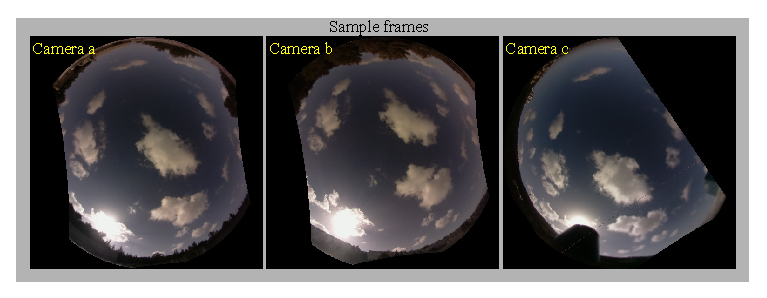
\includegraphics[width=1\linewidth]{figures/projection.eps}
\end{center}
   \vspace{-0.6cm}
   \caption{Frames taken from multiple views, aligned and  shown in polar azimuthal equidistant projection.
   }
\label{fig:inputs}
\end{figure}
To cross-validate 3D recovery, we performed using only four cameras (indexed $a,b,c,d$) out of five cameras. Camera $e$ was ignored. Then, we projected the estimated 3D cloud distribution into viewpoint $e$, and compared to the ground truth. The rendered image is as follows. {\em Ray casting}~\cite{levoycast} of  field $\{T_k\}_k$ is performed on a ray corresponding to $[{\bf l}_e,{\bm \theta}]$. Ray-casting aggregates $\{T_k\}_k$ on all voxels intersected by the ray. The result is a cloud-score image $w[{\bf l}_e,{\bm \theta}]$.

To visualize $w[{\bf l}_e,{\bm \theta}]$, we used it as $\alpha$-map to the estimated sky-background image (Eq.~\ref{eq:SKY}). The alpha-map is
\begin{equation}
 \alpha[{\bf l}_e,{\bm \theta}]=\left\{
      \begin{array}{ll}
      2w[{\bf l}_e,{\bm \theta}]
      & ~~~~{\rm if}~ 2w[{\bf l}_e,{\bm \theta}]<1 \\
      1
      & ~~~~{\rm otherwise}
      \end{array}
      \right.
  \;.
 \label{eq:alpha}
\end{equation}
The rendered image is then
\begin{equation}
 J[{\bf l}_e,{\bm \theta}]=
 \alpha[{\bf l}_e,{\bm \theta}]+(1-\alpha[{\bf l}_e,{\bm \theta}]){\rm SKY}({\bm \theta})
  \;.
 \label{eq:alpha}
\end{equation}
This image does not pretend to properly render clouds in their true shades and effect on the sky. It simply served to visualize the result, as shown in Fig.~\ref{fig:projection}b. It can be compared to the true corresponding image $\hat I_t[{\bf l}_e,{\bm \theta}]$, in Fig.~\ref{fig:projection}c.
\begin{figure}[t!]
\begin{center}
   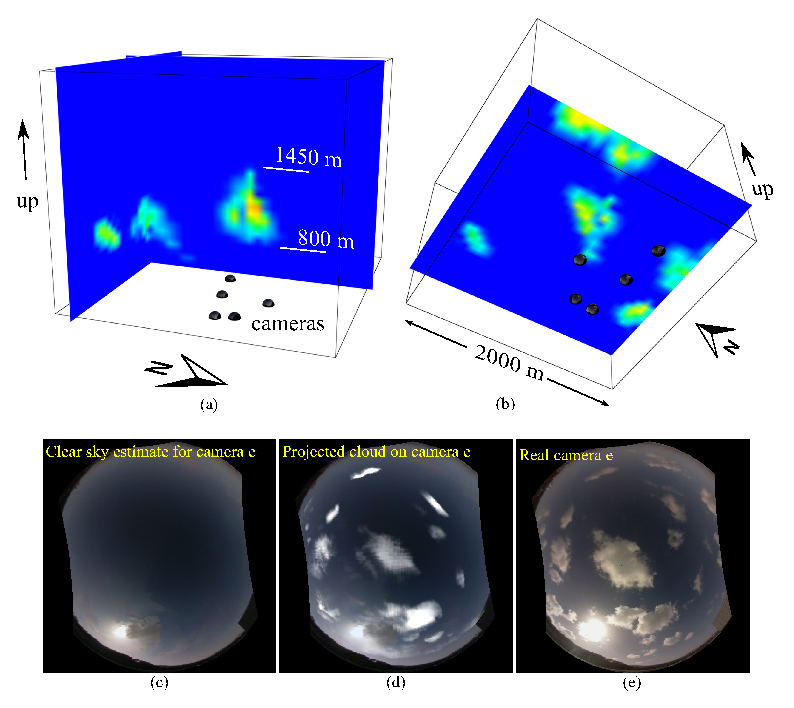
\includegraphics[width=1\linewidth]{figures/clouds_reconstructions.eps}
\end{center}
   \vspace{-0.6cm}
   \caption{3D cloud recovery results. (a,b) Cross-sections of the recovered cloud-occupancy field $\{T_k\}_k$. Note how the domain of the clouds is much larger than the camera network. (c) Estimated sky-background image.  Based on four viewpoints (indexed $a,b,c,d$), the 3D volumetric cloud-occupancy field $\{T_k\}_k$ was derived. The field $\{T_k\}_k$ was projected to viewpoint $e$, and overlayed on the estimated sky-background image. The resulting synthetic cloud-score image $J[{\bf l}_e,{\bm \theta}]$ is shown in (d). This can be compared to the real captured image $\hat I_t[{\bf l}_e,{\bm \theta}]$, shown in (e).}
\label{fig:projection}
\end{figure}

This rendering relies on the redundancy of the network. Even if a viewpoint is blocked, much of its information can be derived using other viewpoints compounded with 3D recovery. This supports the proposed approach for static Sun-blocking (part of the sky missing from a view), described in Sec.~\ref{sec:mutiSun}.

%The pose can be self-calibrated using multiview geometry, particularly {\em structure from motion} (SfM), which has been extensively developed~\cite{birkbeck,cremers,matousek,pollefeys,ruf,woodford} by the computer vision community. A preliminary result is shown in Fig.~\ref{fig:clouds2}, obtained by the Israeli group.
%


%%%%%%%%%%%%%%%%%%%%%%%%%%%%%%%%%%%%%%%%%%%%%%%%%%%%%%%%%%%%%%
\section{Discussion}
\label{sec:discuss}

Scaling light-field imaging hugely to sense the sky, would use  a large network of camera nodes, each having a hemispherical field of view, deployed over a wide area. Such a network can reach anywhere wireless communication exists, and in principle can be a continent-wide light-field system. This sensing approach offers significant advantages over existing technologies (experimental and operational) of atmospheric sensing, particularly  3D imaging, and doing so in high spatio-temporal resolution. This sensing approach poses new questions for computer vision and computational photography. These include network-based extensions to tasks that had been deal with in monocular computer vision. These include network-based radiometric calibration and background estimation. Moreover, network redundancy offers the ability of by-passing blind spots, as those created by sun-blockers, without moving parts.

To enable a massive network, each node should have very low-cost. To demonstrate this can work, we built the units in our experimental small-network using very basic components and coarse alignment tolerances. In a long term, mass producing consistent units would ensure proper alignment performance (non dead-regions), operational robustness over long periods. Still, this concept opens the door to more interesting research. In the direction of the sun blocker, a diffraction grating can disperse direct sunlight (currently blocked) or skylight, to measure their spectra. This principle is already used by Aeronet~\cite{aeronet} to characterize aersols. Night-time operation is another interesting challenge: if a known planet and star appears missing on ray $r$, this indicated a cloud on $r$. Furthermore, such a light-field system can be used for studying lightnings and bird life, in 3D time-lapses.





\bibliographystyle{splncs}
\bibliography{MyRefs3}
\end{document}
